\section{Theory} \label{sec:theory}
To calculate the energies, we need to solve the Schrödinger equation
\begin{equation}
\hat{H}\ket{\Psi_p}=\varepsilon_p\ket{\Psi_p}
\end{equation}
where we expect to find the exact ground state energy, $\varepsilon_0$, when the correct ground state wave function (GSWF) has been used. In this project we will stick to the Born-Oppenheimer approximation, which gives the Hamiltonian when the nucleus is stationary (is not affected by the electrons),
\begin{equation}
\hat{H}=\sum_{i=1}^Nt(x_i)-\sum_{i=1}^Nk\frac{Ze^2}{r_i}+\sum_{i<j}^N\frac{ke^2}{r_{ij}}.
\end{equation}
The first term gives the kinetic energy, the second gives the energy from the external potential (nucleus) and the last term gives the interaction energy. $Z$ is the atomic number, defining the number of protons in the nucleus, $k$ is the constant from Coulomb's law and $e$ is the elementary change.

We now introduce the atomic units, setting $\hbar=c=e=m_e=k=1$. 
The energies can be converted between atomic units and electronvolts using the relation
\begin{equation}
1 \text{ a.u.} = 2\cdot13.6 \text{ eV}.
\end{equation}
The Hamiltonian now reads
\begin{equation}
\hat{H}=\hat{H}_0 + \hat{H}_I=\sum_{i=1}^N\hat{h}_0(x_i)+\sum_{i<j}^N\frac{1}{r_{ij}}
\end{equation}
with $r_{ij}\equiv\frac{1}{|\boldsymbol{r}_i-\boldsymbol{r}_j|}$ and $\hat{h}_0$ as the one-body operator for each electron. The single particle functions (SPF) are assumed to be hydrogen-like, where the one-body energies are known from the Bohr model, stating
\begin{equation}
E_n=-\frac{Z^2}{2n^2}
\end{equation}
where $n$ is the number of nodes in the wave function. In order to calculate the two-body energies, we need to solve the integrals 
\begin{equation}
\int r_1^2dr_1\int r_2^2dr_2 \Phi_{\alpha}^*(r_1)\Phi_{\beta}^*(r_2)\frac{1}{|\boldsymbol{r}_1-\boldsymbol{r}_2|}\Phi_{\gamma}(r_1)\Phi_{\delta}(r_2)\equiv\mel{\alpha\beta}{\hat{v}}{\gamma\delta}
\end{equation}
where the Dirac notation is used for shorthand notation. Note carefully that the $\Phi$'s are the total wave functions, where both the radial and spin parts are included. The spin part is known to not affect the energies, and it can therefore be factorized out,
\begin{align}
\mel{\alpha\beta}{\hat{v}}{\gamma\delta}&=(\alpha\beta|\hat{v}|\gamma\delta)\braket{\chi_{\alpha}\chi_{\beta}}{\chi_{\gamma}\chi_{\delta}}\notag\\
&=(\alpha\beta|\hat{v}|\gamma\delta)\braket{\chi_{\alpha}}{\chi_{\gamma}}\braket{\chi_{\beta}}{\chi_{\delta}}\\
&=(\alpha\beta|\hat{v}|\gamma\delta)\,\delta_{\sigma_{\alpha}\sigma_{\gamma}}\delta_{\sigma_{\beta}\sigma_{\delta}}.\notag
\end{align}
We observe that the integral is non-zero if and only if $\alpha$ and $\gamma$ got the same spin, and $\beta$ and $\delta$ got the same spin.

\subsection{Second Quantization and particle-hole-formalism}
First write some general second quantization statements, when define the Hamiltonian in second quantization

\subsubsection{Wick's theorem}
State Wick's theorem 

\subsubsection{Energy formulas}
For calculating the ground state energy of an atom with atomic number $Z$, we need to calculate
\begin{align}
	\varepsilon_0=\mel{\Phi_0}{\hat{H}}{\Phi_0}&=\sum_i\mel{i}{\hat{h}_0}{i}+\frac{1}{2}\sum_{ij}\mel{ij}{\hat{v}}{ij}_{\text{AS}}\label{eq:E_ref}
\end{align}
where the subscript AS...
See appendix A. 
Should also add cHia and iaHja, and mention that they are gonna be used in CIS.

\subsection{The Helium atom}
A neutral Helium atom consists of a nucleus of two protons with two electrons orbiting, and is one of the most simple many-body systems one can study. The difficulty of dealing with many-body systems lies in the interaction, where the elements $\mel{\alpha\beta}{\hat{v}}{\gamma\delta}$ can be really tricky to handle. Hard to find exact wave function. 

There exist various methods for solving this problem, where one of the most successful is to define a wave function which is varied such that the energy is minimized. This method was used by E. Hylleraas already in 1929, when he minimized the energy with a wave function of 10 variational parameters, using a mechanical desk calculator. [https://www.encyclopedia.com/science/dictionaries-thesauruses-pictures-and-press-releases/hylleraas-egil-andersen] He found the energy to be -2.90363 eV, which is close to recent experimental values. [http://www.umich.edu/~chem461/QMChap8.pdf][https://journals.aps.org/prl/abstract/10.1103/PhysRevLett.80.3475]. 




Lide 1992
Handbook of Chem. and Phys. lide 1992



\subsubsection{Ground state}
Helium is in its ground state when both electrons occupy the 1s orbital, thus they have opposite spins and $M_s=0$. In this project, we will study systems of $M_s=0$ only, such that an electron can only be excited to a state with the same spin. 

Taking the Pauli principle into account, the two-body wavefunction needs to be nulled out if two particles are in the same state, and it should also be antisymmetric under exchange of two particles. We are therefore in need of a Slater Determinant (SD), given by
\begin{align}
	\Psi(x_1,x_2,\sigma_1,\sigma_2)&=A\mqty|\psi_{\sigma_1}(x_1) & \psi_{\sigma_1}(x_2)\\ \psi_{\sigma_2}(x_1) & \psi_{\sigma_2}(x_2)|\\
	&=A\Big[\psi_{\sigma_1}(x_1)\psi_{\sigma_2}(x_2)-\psi_{\sigma_2}(x_1)\psi_{\sigma_1}(x_2)\Big]
\end{align}
where $\psi_{\sigma_1}$ is the SPF with spin $m_s=\sigma_1$ and $A$ is a normalization constant. If we assume that the SPFs are normalized, our ansatz can be written as
\begin{equation}
\ket{\Phi_0}=\frac{1}{\sqrt{2}}(\ket{1}\ket{\bar{1}}-\ket{\bar{1}}\ket{1})
\end{equation}
with $\ket{\bar{1}}$ describing a particle with principle quantum number 1 and spin $\sigma_2$, which we will illustrate with spin down. In second quantization, we can construct the ground state from the true vacuum,
\begin{equation}
\ket{\Phi_0}=a_{1}^{\dagger}a_{\bar{1}}^{\dagger}\ket{0},
\end{equation}
which is understand to take the anti-symmetry property. The ground state is illustrated in figure \eqref{fig:schematic_he_gs}.
\begin{figure} [H]
	\begin{center}
		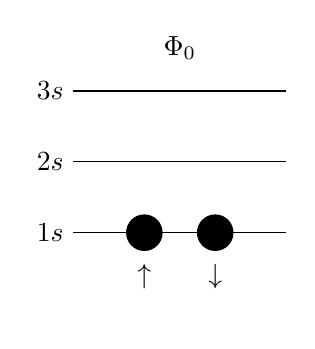
\begin{tikzpicture}[scale=0.9]
		\begin{scope}
			\foreach \i in {1,...,3}
			{
				\draw (-1,\i-1) node[anchor=east] {$\i s$} --(2,\i-1);
			}
			\filldraw (0,0) node[anchor=north,inner sep=.4cm] {$\uparrow$} circle (0.25cm); 
			\filldraw (1,0) node[anchor=north,inner sep=.4cm] {$\downarrow$} circle (0.25cm);
			\node[] at (0.5,2.6) {$\ket{\Phi_0}$};
		\end{scope}
		\end{tikzpicture}
	\end{center}
\caption{Ground state of Helium.}
\label{fig:schematic_he_gs}
\end{figure}

\subsubsection{Excited states}
When entering excited states, we can risk having angular quantum numbers unlike zero, because $l\in[0,n-1]$. This makes the computations more difficult, but in this project we will ignore that challenge setting $l=0$, and thus limit us to the s-waves. 

Consider now a system consisting of the orbitals 1s, 2s and 3s only. For that case, the possible energy states of the Helium atom are listed in figure \eqref{fig:schematic_he}.
\begin{figure} [H]
	\begin{center}
		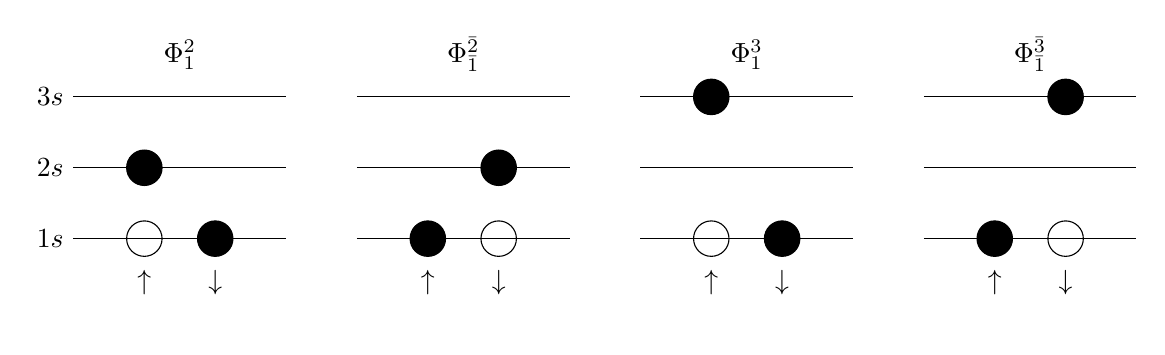
\begin{tikzpicture}[scale=0.9]
		\begin{scope}
		\foreach \i in {1,...,3}
		{
			\draw (-1,\i-1) node[anchor=east] {$\i s$} --(2,\i-1);
		}
		\draw (0,0) node[anchor=north,inner sep=.4cm] {$\uparrow$} circle (0.25cm); 
		\filldraw (1,0) node[anchor=north,inner sep=.4cm] {$\downarrow$} circle (0.25cm);
		\filldraw (0,1) circle (0.25cm);
		\node[] at (0.5,2.6) {$\ket{\Phi_{1}^{2}}$};
		\end{scope}
		\begin{scope}[xshift=4cm]
		\foreach \i in {1,...,3}
		{
			\draw (-1,\i-1) --(2,\i-1);
		}
		\filldraw (0,0) node[anchor=north,inner sep=.4cm] {$\uparrow$} circle (0.25cm); 
		\draw (1,0) node[anchor=north,inner sep=.4cm] {$\downarrow$} circle (0.25cm);
		\filldraw (1,1) circle (0.25cm);
		\node[] at (0.5,2.6) {$\ket{\Phi_{\bar{1}}^{\bar{2}}}$};
		\end{scope}
		\begin{scope}[xshift=8cm]
		\foreach \i in {1,...,3}
		{
			\draw (-1,\i-1) --(2,\i-1);
		}
		\draw (0,0) node[anchor=north,inner sep=.4cm] {$\uparrow$} circle (0.25cm); 
		\filldraw (1,0) node[anchor=north,inner sep=.4cm] {$\downarrow$} circle (0.25cm);
		\filldraw (0,2) circle (0.25cm); 
		\node[] at (0.5,2.6) {$\ket{\Phi_{1}^{3}}$};
		\end{scope}
		\begin{scope}[xshift=12cm]
		\foreach \i in {1,...,3}
		{
			\draw (-1,\i-1) --(2,\i-1);
		}
		\filldraw (0,0) node[anchor=north,inner sep=.4cm] {$\uparrow$} circle (0.25cm); 
		\draw (1,0) node[anchor=north,inner sep=.4cm] {$\downarrow$} circle (0.25cm);
		\filldraw (1,2) circle (0.25cm); 
		\node[] at (0.5,2.6) {$\ket{\Phi_{\bar{1}}^{\bar{3}}}$};
		\end{scope}
		\end{tikzpicture}
		\newline
		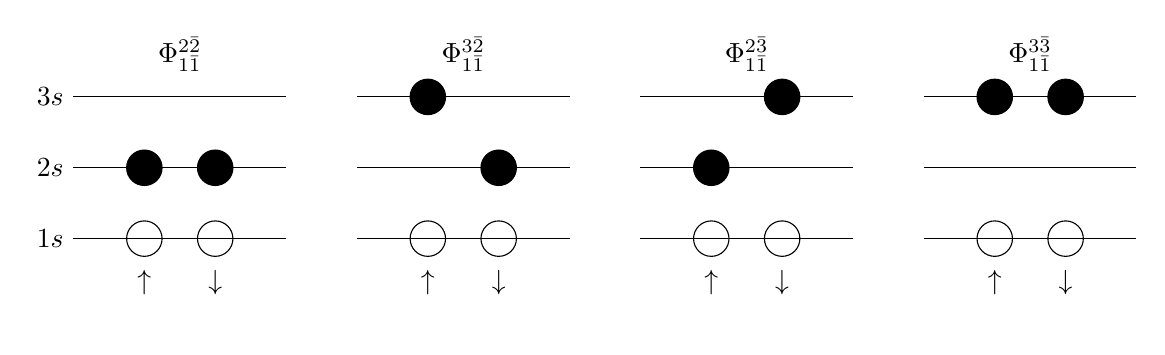
\begin{tikzpicture}[scale=0.9]
		\begin{scope}
		\foreach \i in {1,...,3}
		{
			\draw (-1,\i-1) node[anchor=east] {$\i s$} --(2,\i-1);
		}
		\draw (0,0) node[anchor=north,inner sep=.4cm] {$\uparrow$} circle (0.25cm); 
		\draw (1,0) node[anchor=north,inner sep=.4cm] {$\downarrow$} circle (0.25cm);
		\filldraw (0,1) circle (0.25cm);
		\filldraw (1,1) circle (0.25cm);
		\node[] at (0.5,2.6) {$\ket{\Phi_{1\bar{1}}^{2\bar{2}}}$};
		\end{scope}
		\begin{scope}[xshift=4cm]
		\foreach \i in {1,...,3}
		{
			\draw (-1,\i-1) --(2,\i-1);
		}
		\draw (0,0) node[anchor=north,inner sep=.4cm] {$\uparrow$} circle (0.25cm); 
		\draw (1,0) node[anchor=north,inner sep=.4cm] {$\downarrow$} circle (0.25cm);
		\filldraw (0,2) circle (0.25cm); 
		\filldraw (1,1) circle (0.25cm); 
		\node[] at (0.5,2.6) {$\ket{\Phi_{1\bar{1}}^{3\bar{2}}}$};
		\end{scope}
		\begin{scope}[xshift=8cm]
		\foreach \i in {1,...,3}
		{
			\draw (-1,\i-1) --(2,\i-1);
		}
		\draw (0,0) node[anchor=north,inner sep=.4cm] {$\uparrow$} circle (0.25cm); 
		\draw (1,0) node[anchor=north,inner sep=.4cm] {$\downarrow$} circle (0.25cm);
		\filldraw (1,2) circle (0.25cm);
		\filldraw (0,1) circle (0.25cm);
		\node[] at (0.5,2.6) {$\ket{\Phi_{1\bar{1}}^{2\bar{3}}}$};
		\end{scope}
		\begin{scope}[xshift=12cm]
		\foreach \i in {1,...,3}
		{
			\draw (-1,\i-1) --(2,\i-1);
		}
		\draw (0,0) node[anchor=north,inner sep=.4cm] {$\uparrow$} circle (0.25cm); 
		\draw (1,0) node[anchor=north,inner sep=.4cm] {$\downarrow$} circle (0.25cm);
		\filldraw (0,2) circle (0.25cm); 
		\filldraw (1,2) circle (0.25cm);
		\node[] at (0.5,2.6) {$\ket{\Phi_{1\bar{1}}^{3\bar{3}}}$};
		\end{scope}
		\end{tikzpicture}
	\end{center}
	\caption{Possible states in the 1s, 2s and 3s orbitals of Helium. In the first row, all single excited states are listed, while in the second row all double excited states are listed.}
	\label{fig:schematic_he}
\end{figure}

\subsection{The Beryllium atom}

\subsubsection{Ground state}
Helium is in its ground state when both electrons occupy the 1s orbital, thus they have opposite spins and $M_s=0$. In this project, we will study systems of $M_s=0$ only, such that an electron can only be excited to a state with the same spin. 

Taking the Pauli principle into account, the two-body wavefunction needs to be nulled out if two particles are in the same state, and it should also be antisymmetric under exchange of two particles. We are therefore in need of a Slater Determinant (SD), given by
\begin{align}
\Psi(x_1,x_2,\sigma_1,\sigma_2)&=A\mqty|\psi_{\sigma_1}(x_1) & \psi_{\sigma_1}(x_2)\\ \psi_{\sigma_2}(x_1) & \psi_{\sigma_2}(x_2)|\\
&=A\Big[\psi_{\sigma_1}(x_1)\psi_{\sigma_2}(x_2)-\psi_{\sigma_2}(x_1)\psi_{\sigma_1}(x_2)\Big]
\end{align}
where $\psi_{\sigma_1}$ is the SPF with spin $m_s=\sigma_1$ and $A$ is a normalization constant. If we assume that the SPFs are normalized, our ansatz can be written as
\begin{equation}
\ket{\Phi_0}=\frac{1}{\sqrt{2}}(\ket{1}\ket{\bar{1}}-\ket{\bar{1}}\ket{1})
\end{equation}
with $\ket{\bar{1}}$ describing a particle with principle quantum number 1 and spin $\sigma_2$, which we will illustrate with spin down. In second quantization, we can construct the ground state from the true vacuum,
\begin{equation}
\ket{\Phi_0}=a_{1}^{\dagger}a_{\bar{1}}^{\dagger}\ket{0},
\end{equation}
which is understand to take the anti-symmetry property. The ground state is illustrated in figure \eqref{fig:schematic_he_gs}.
\begin{figure} [H]
	\begin{center}
		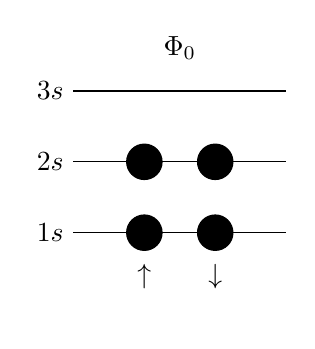
\begin{tikzpicture}[scale=0.9]
		\begin{scope}
		\foreach \i in {1,...,3}
		{
			\draw (-1,\i-1) node[anchor=east] {$\i s$} --(2,\i-1);
		}
		\filldraw (0,0) node[anchor=north,inner sep=.4cm] {$\uparrow$} circle (0.25cm); 
		\filldraw (1,0) node[anchor=north,inner sep=.4cm] {$\downarrow$} circle (0.25cm);
		\filldraw (0,1) circle (0.25cm);
		\filldraw (1,1) circle (0.25cm);
		\node[] at (0.5,2.6) {$\ket{\Phi_0}$};
		\end{scope}
		\end{tikzpicture}
	\end{center}
	\caption{Ground state of Beryllium.}
	\label{fig:schematic_be_gs}
\end{figure}

\subsubsection{Excited states}
When entering excited states, we can risk having angular quantum numbers unlike zero, because $l\in[0,n-1]$. This makes the computations more difficult, but in this project we will ignore that challenge setting $l=0$, and thus limit us to the s-waves. 

Consider now a system consisting of the orbitals 1s, 2s and 3s only. For that case, the possible energy states of the Helium atom are listed in figure \eqref{fig:schematic_he}.
\begin{figure} [H]
	\begin{center}
		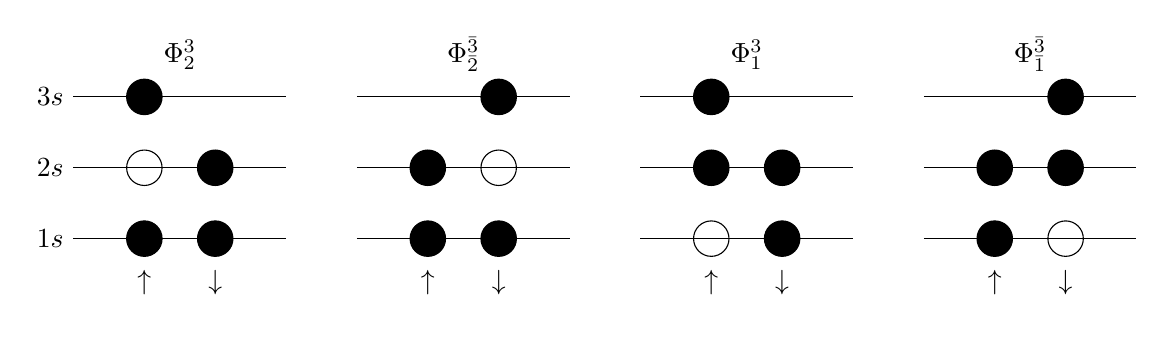
\begin{tikzpicture}[scale=0.9]
		\begin{scope}
		\foreach \i in {1,...,3}
		{
			\draw (-1,\i-1) node[anchor=east] {$\i s$} --(2,\i-1);
		}
		\filldraw (0,0) node[anchor=north,inner sep=.4cm] {$\uparrow$} circle (0.25cm); 
		\filldraw (1,0) node[anchor=north,inner sep=.4cm] {$\downarrow$} circle (0.25cm);
		\draw (0,1) circle (0.25cm);
		\filldraw (1,1) circle (0.25cm);
		\filldraw (0,2) circle (0.25cm);
		\node[] at (0.5,2.6) {$\ket{\Phi_2^3}$};
		\end{scope}
		\begin{scope}[xshift=4cm]
		\foreach \i in {1,...,3}
		{
			\draw (-1,\i-1) --(2,\i-1);
		}
		\filldraw (0,0) node[anchor=north,inner sep=.4cm] {$\uparrow$} circle (0.25cm); 
		\filldraw (1,0) node[anchor=north,inner sep=.4cm] {$\downarrow$} circle (0.25cm);
		\draw (1,1) circle (0.25cm);
		\filldraw (1,2) circle (0.25cm);
		\filldraw (0,1) circle (0.25cm);
		\node[] at (0.5,2.6) {$\ket{\Phi_{\bar{2}}^{\bar{3}}}$};
		\end{scope}
		\begin{scope}[xshift=8cm]
		\foreach \i in {1,...,3}
		{
			\draw (-1,\i-1) -- (2,\i-1);
		}
		\draw (0,0) node[anchor=north,inner sep=.4cm] {$\uparrow$} circle (0.25cm); 
		\filldraw (1,0) node[anchor=north,inner sep=.4cm] {$\downarrow$} circle (0.25cm);
		\filldraw (0,1) circle (0.25cm);
		\filldraw (1,1) circle (0.25cm);
		\filldraw (0,2) circle (0.25cm);
		\node[] at (0.5,2.6) {$\ket{\Phi_{1}^{3}}$};
		\end{scope}
		\begin{scope}[xshift=12cm]
		\foreach \i in {1,...,3}
		{
			\draw (-1,\i-1) --(2,\i-1);
		}
		\filldraw (0,0) node[anchor=north,inner sep=.4cm] {$\uparrow$} circle (0.25cm); 
		\draw (1,0) node[anchor=north,inner sep=.4cm] {$\downarrow$} circle (0.25cm);
		\filldraw (1,1) circle (0.25cm);
		\filldraw (1,2) circle (0.25cm);
		\filldraw (0,1) circle (0.25cm);
		\node[] at (0.5,2.6) {$\ket{\Phi_{\bar{1}}^{\bar{3}}}$};
		\end{scope}
		\end{tikzpicture}
		\newline
		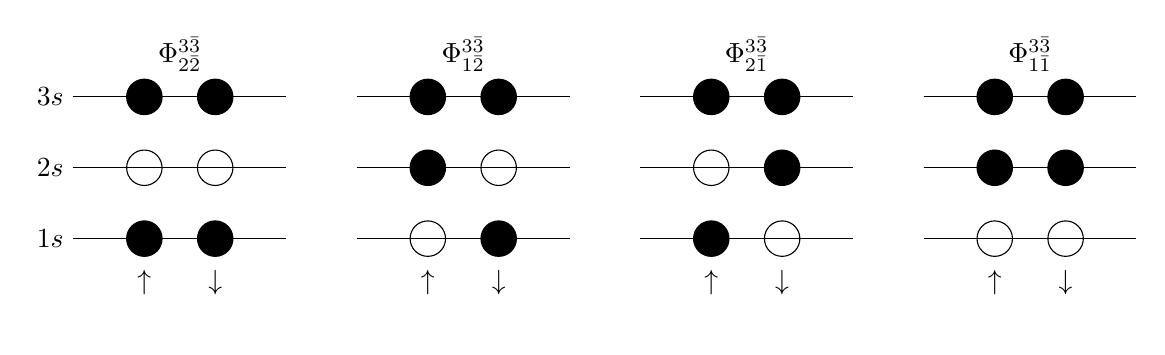
\begin{tikzpicture}[scale=0.9]
		\begin{scope}
		\foreach \i in {1,...,3}
		{
			\draw (-1,\i-1) node[anchor=east] {$\i s$} --(2,\i-1);
		}
		\filldraw (0,0) node[anchor=north,inner sep=.4cm] {$\uparrow$} circle (0.25cm); 
		\filldraw (1,0) node[anchor=north,inner sep=.4cm] {$\downarrow$} circle (0.25cm);
		\draw (0,1) circle (0.25cm);
		\draw (1,1) circle (0.25cm);
		\filldraw (0,2) circle (0.25cm);
		\filldraw (1,2) circle (0.25cm);
		\node[] at (0.5,2.6) {$\ket{\Phi_{2\bar{2}}^{3\bar{3}}}$};
		\end{scope}
		\begin{scope}[xshift=4cm]
		\foreach \i in {1,...,3}
		{
			\draw (-1,\i-1) --(2,\i-1);
		}
		\draw (0,0) node[anchor=north,inner sep=.4cm] {$\uparrow$} circle (0.25cm); 
		\filldraw (1,0) node[anchor=north,inner sep=.4cm] {$\downarrow$} circle (0.25cm);
		\draw (1,1) circle (0.25cm);
		\filldraw (1,2) circle (0.25cm);
		\filldraw (0,2) circle (0.25cm);
		\filldraw (0,1) circle (0.25cm);
		\node[] at (0.5,2.6) {$\ket{\Phi_{1\bar{2}}^{3\bar{3}}}$};
		\end{scope}
		\begin{scope}[xshift=8cm]
		\foreach \i in {1,...,3}
		{
			\draw (-1,\i-1) -- (2,\i-1);
		}
		\filldraw (0,0) node[anchor=north,inner sep=.4cm] {$\uparrow$} circle (0.25cm); 
		\draw (1,0) node[anchor=north,inner sep=.4cm] {$\downarrow$} circle (0.25cm);
		\draw (0,1) circle (0.25cm);
		\filldraw (1,1) circle (0.25cm);
		\filldraw (0,2) circle (0.25cm);
		\filldraw (1,2) circle (0.25cm);
		\node[] at (0.5,2.6) {$\ket{\Phi_{2\bar{1}}^{3\bar{3}}}$};
		\end{scope}
		\begin{scope}[xshift=12cm]
		\foreach \i in {1,...,3}
		{
			\draw (-1,\i-1) --(2,\i-1);
		}
		\draw (0,0) node[anchor=north,inner sep=.4cm] {$\uparrow$} circle (0.25cm); 
		\draw (1,0) node[anchor=north,inner sep=.4cm] {$\downarrow$} circle (0.25cm);
		\filldraw (1,1) circle (0.25cm);
		\filldraw (1,2) circle (0.25cm);
		\filldraw (0,1) circle (0.25cm);
		\filldraw (0,2) circle (0.25cm);
		\node[] at (0.5,2.6) {$\ket{\Phi_{1\bar{1}}^{3\bar{3}}}$};
		\end{scope}
		\end{tikzpicture}
	\end{center}
	\caption{Possible states in the 1s, 2s and 3s orbitals of Beryllium. In the first row, all single excited states are listed, while in the second row all double excited states are listed.}
	\label{fig:schematic}
\end{figure}